\documentclass[11pt]{article}
\usepackage[margin=1in]{geometry}
\usepackage{amsmath,amssymb,amsthm,graphicx,booktabs,hyperref}
\newtheorem{theorem}{Theorem}
\newtheorem{lemma}[theorem]{Lemma}
\newtheorem{proposition}[theorem]{Proposition}
\newcommand{\Rop}{\operatorname{Rop}}
\newcommand{\Thi}{\operatorname{Thi}}
\title{Staggered toroidal shell blocks:\\a constructive ropelength bound and its first block correction}
\author{Tight Knots Lab --- research draft}
\date{13 September 2026; literature cutoff 12 September 2026}
\begin{document}
\maketitle
\begin{abstract}
We give explicit unit-thickness representatives of the full-twist links
$T(M,M)$ with
$\limsup_{M\to\infty}\Rop(T(M,M))/[M(M-1)]^{3/4}<10.614$.
The construction combines shell-specific conservative capacities with blocks
of equally populated toroidal helices. Alternating half-step phases allow
radial spacing $\sqrt3$ within blocks; block boundaries retain spacing two.
An exact separation estimate and a full-twist cabling argument certify the
geometry and topology. For a block size $b$ among $T$ shells, the normalized
constructed length has an expansion
$\alpha[1+a/b+d b/T+O(b^{-2}+(b/T)^2+T^{-1})]$.
In the regime $b\to\infty$, $b/T\to0$, its first correction among $b=\lfloor c\sqrt T\rfloor$ is uniquely minimized
at an explicitly defined integral constant $c_*\approx0.422785$.
The results concern upper constructions and a specified block grammar;
neither global ropelength optimality nor publication priority is asserted.
\end{abstract}

\section{Conventions, context and scope}
Thickness is tube radius and the length of a link is the sum of its component
lengths. For smooth embedded closed curves, thickness is the minimum of the
curvature radius and half the doubly critical self-distance, including
intercomponent separation for a union \cite{cks}. Our curves are smooth;
polygonal computations used for controls are not substituted for their reach.
The crossing number of $T(M,M)$ is $M(M-1)$.

Concentric helices, toroidal bending, shell population choices and torus-hole
doubling occur in the work of Klotz and Thompson \cite{kt25,klotz26}.
Toroidal and hexagonal filament packings have older precedents
\cite{ob12,star06,atkinson19}. These ingredients are not claimed as new.
The focused contribution considered here is the exact shell-specific
capacity, block phase compatibility, and their quantitative limiting and
boundary-error analysis. In particular, reciprocal-plus-linear optimization
and a square-root shell scale already occur in \cite[Eq.\ (17)--(18)]{kt25}.
The possible distinction is the geometry-specific expansion proved below.
The bounded prior-art audit accompanying this draft labels publication
novelty \emph{possibly novel}, not established priority.

Klotz's common-hole optimized coefficient near $11.68$ is conditional on its
no-overlap approximation \cite{klotz26}. Our comparison preserves that
qualification. No universal lower-bound improvement, matching asymptotic
lower bound, or best-known record across other torus families is claimed.

\section{Finite construction and clearance}
For $R>r>0$ and a phase $\phi$ put
\begin{equation}\label{curve}
F_{r,\phi}(t)=((R+r\cos t)\cos(t+\phi),
 (R+r\cos t)\sin(t+\phi),r\sin t),\quad t\in\mathbb R/(2\pi\mathbb Z).
\end{equation}
Write $h=R-r$ and $A(r,h)=\pi rh/\sqrt{r^2+h^2}$.

\begin{lemma}\label{same}
If $r\ge2$, $R\ge2r+2$, and $N=\lfloor A(r,R-r)\rfloor-1$,
the $N$ curves with phases $2\pi j/N$ have pairwise distance at least two.
Each has thickness at least one.
\end{lemma}
\begin{proof}
Here $N\ge4$ since $r\ge2$, $h\ge4$ and $A\ge8\pi/\sqrt{20}>5$.
For parameter difference $u=t-s$ and phase difference $\Delta$, direct
expansion gives
\[
 |F_{r,\phi}(t)-F_{r,\psi}(s)|^2
 =4r^2\sin^2(u/2)+4(R+r\cos t)(R+r\cos s)
                  \sin^2((u+\Delta)/2).
\]
Replacing the positive radial product by $h^2$ and combining cosines bounds
this below by $2(S-\sqrt{S^2-4r^2h^2\sin^2(\Delta/2)})$, where
$S=r^2+h^2$. This is at least four if
$r^2h^2\sin^2(\Delta/2)\ge S-1$. The least nonzero phase has
$\sin^2(\Delta/2)\ge\sin^2(\pi/N)$. For $N\ge3$,
$\sin(\pi/N)\ge\pi/(N+1)$: use
$\sin x\ge x-x^3/6$ and $\pi^2(N+1)\le6N^2$.
Our choice $N+1\le A$ consequently gives the stronger lower bound $S$.

For one curve $|F'|\ge h$ and $|F''|\le B=R+\sqrt5r$.
Since $r\le h-2$, $h\ge4$ and $\sqrt5<9/4$,
$B/h^2\le17/(4h)-6/h^2\le11/16$; curvature is at most $11/16$.
A doubly critical chord with shorter cyclic separation $0<u\le\pi$
satisfies $u\ge2h/B$ by Taylor's integral remainder applied to its scalar
product with $F'(s)$. The displayed distance identity with $\Delta=0$
therefore gives chord length at least
$2h\sin(h/B)\ge(5/3)h^2/B\ge80/33>2$.
The longitude is one-to-one and cylindrical radius positive, proving
embeddedness. The smooth thickness formula completes the proof.
\end{proof}

\begin{lemma}\label{cross}
For shell radii $u\le v<R/2$ and any phase difference $\Delta$, all point
pairs have squared distance at least
\[
 (u-v)^2+4K\sin^2(\Delta/2),\qquad
 K=\frac{uv(R-u)(R-v)}{uv+(R-u)(R-v)}.
\]
For $0<r_0\le u\le v<R/2$, consider a block with common population $N=\lfloor A(r_0,R-r_0)\rfloor-1$,
$r_0$ its first radius and $N\ge3$. Alternating phase offsets $0,\pi/N$ permit
neighboring radial spacing $\sqrt3$.
\end{lemma}
\begin{proof}
The transverse squared term is
$(u-v)^2+4uv\sin^2((t-s)/2)$; the remaining radial product is at least
$(R-u)(R-v)$. The same harmonic minimization gives
$2(S-\sqrt{S^2-4P\sin^2(\Delta/2)})$, with
$S=uv+(R-u)(R-v)$, $P=uv(R-u)(R-v)$.
Rationalizing, or using $\sqrt{1-z}\le1-z/2$, bounds this by
$4(P/S)\sin^2(\Delta/2)$ from below.

For $u\le v<R/2$, the reciprocal
$1/K=1/(uv)+1/((R-u)(R-v))$ decreases as $v$ increases;
its derivative is negative since
$(R-u)(R-v)^2>uv^2$. The diagonal value increases with $u<R/2$.
Thus $K\ge K(r_0,r_0)=A(r_0,R-r_0)^2/\pi^2$.
For adjacent shells every phase difference is an odd multiple of $\pi/N$.
Applying the sine inequality with $2N$ yields
\[
4K\sin^2(\Delta/2)\ge\frac{4(N+1)^2}{(2N+1)^2}>1.
\]
Adding radial squared gap three proves the assertion.
\end{proof}

Choose integers $T\ge1$, $1\le b\le T$, let $\delta=\sqrt3$, $g=2-\delta$,
and set
\begin{align}\label{grammar}
r_i&=\delta i+g\lceil i/b\rceil,& R&=2r_T+2,\\
j(i)&=1+b\lfloor(i-1)/b\rfloor,&
N_i&=\lfloor A(r_{j(i)},R-r_{j(i)})\rfloor-1.\nonumber
\end{align}
On each shell use equally spaced phases with offsets alternating $0,\pi/N_i$
inside its block. Include the core $C(t)=(R\cos t,R\sin t,0)$.
There are $Q=1+\sum_iN_i$ components in this bundle. Duplicate the entire
bundle by the proper rigid motion $P(x,y,z)=(R+x,-z,y)$, giving $M=2Q$.

\begin{proposition}\label{finite}
For every stated $T,b$, this construction has thickness at least one and
link type $T(2Q,2Q)$ up to a common mirror.
\end{proposition}
\begin{proof}
The first radius is two. Lemmas \ref{same}--\ref{cross} cover same-shell
and adjacent within-block pairs. The common block population is conservative
for its other shells because $A(r,R-r)$ increases for $r<R/2$.
Nonadjacent shells have radial gap at least $2\sqrt3$, and block boundaries
have gap two; the transverse distance alone suffices in these cases.
Each shell has distance $r_i$ from its core. The two round Hopf cores have
minimum distance $R$, as is seen from
\[
|C(t)-P(C(s))|^2=R^2[1+2(1-\cos t)(1+\cos s)]\ge R^2.
\]
Every component lies within $r_T$ of its core, so every cross-bundle pair
has distance at least $R-2r_T=2$. The self-thickness estimate applies since
$R\ge2r_i+2$.

For topology use zero-framed tubular coordinates
$E(u,a+ib)=((R+a)\cos u,(R+a)\sin u,b)$.
Writing $u=t+\phi$, every strand is $E(u,e^{iu}w)$ for a fixed distinct
point $w=r e^{-i\phi}$, including $w=0$ for the core. A path of distinct
disk configurations induces an isotopy of the link; move these points to a
small circle to obtain the closure of the full twist on $Q$ strands.
The radial/vertical frame is the zero framing: a fixed radial push-off is a
planar circle with linking number zero.

To check the doubling, rotate two small disjoint point clusters once.
The paths $e^{iu}(c_k+w_{kj})$ factor into rotation of their centers and
internal rotation of each cluster. Independent center and internal angles
range over a square of collision-free configurations; its diagonal is
homotopic to its two edges. Thus a full twist on $2Q$ points factors as
the internal full twists and the zero-framed mutual Hopf twist.
The explicit core arrangement is the standard round Hopf link. Signs agree:
a first-bundle helix pierces its core's positively oriented spanning disk
once downward, and the second core also pierces that disk once downward.
The proper motion preserves the other internal sign. Hence this geometric
cabling is the full twist on $2Q$ strands, up to a common mirror.
This is a configuration-space and framing proof, not identification by
pairwise linking numbers alone.
\end{proof}

\section{Leading coefficient and a uniform first correction}
Define smooth functions and constants
\begin{align*}
n(x)&=\frac{2\pi x(2-x)}{\sqrt{x^2+(2-x)^2}},&
e(x)&=\int_0^{2\pi}\sqrt{(4+2x\cos t)^2+4x^2}\,dt,\\
q_0&=\int_0^1n(x)\,dx
=\pi\left(\frac{3\operatorname{arsinh}(1)}{\sqrt2}-1\right),&
l_0&=\int_0^1n(x)e(x)\,dx,\\
n_1&=n(1)=\sqrt2\pi,& J&=\int_0^1n'(x)e(x)\,dx,\\
\alpha&=\sqrt{\delta/2}\,\frac{l_0}{\sqrt2q_0^{3/2}},&
a&=\frac{g}{2\delta},\qquad d=\frac{3n_1}{4q_0}-\frac{J}{2l_0}.
\end{align*}
Let $L(T,b)$ be the exact total analytic length in Proposition \ref{finite},
and $F(T,b)=L(T,b)/[M(T,b)(M(T,b)-1)]^{3/4}$.

\begin{theorem}\label{correction}
As $b\to\infty$ and $b/T\to0$ through admissible integers,
\begin{equation}\label{expansion}
F(T,b)=\alpha\left[1+\frac{a}{b}+\frac{db}{T}
 +O\left(b^{-2}+(b/T)^2+T^{-1}\right)\right],
\end{equation}
with uniform implied constants in that regime. For fixed $c>0$ and
$b=\lfloor c\sqrt T\rfloor$ the coefficient of $T^{-1/2}$ is
$\beta(c)=\alpha(a/c+dc)$. It is uniquely minimized at $c_* =\sqrt{a/d}<1$,
with $\beta_*=2\alpha\sqrt{ad}<\beta(1)$.
\end{theorem}
\begin{proof}
Put $\lambda=\delta+g/b$. The exact difference
$r_i-\lambda i=g(\lceil i/b\rceil-i/b)$ lies in $[0,g)$, including the
incomplete last block. Therefore, uniformly in $i,T,b$,
\[
r_i=\lambda i+O(1),\quad R=2\lambda T+O(1),\quad
N_i=\frac{\lambda T}{2}n(j(i)/T)+O(1),\quad
\ell_i=\frac{\lambda T}{2}e(i/T)+O(1).
\]
Here $\ell_i$ is one shell component's length. The last two estimates follow
from homogeneity, bounded first derivatives of the capacity and speed
integral, and an error of less than two for flooring and subtracting one.
For example $|\partial_r A|,|\partial_h A|\le\pi$,
$|\partial_R\ell|\le2\pi$, $|\partial_r\ell|\le2\pi\sqrt2$.
These estimates remain valid at the innermost shells.

Write $k_i=i-j(i)$. For any fixed $C^1$ function $h$ on $[0,1]$,
\[
\sum_i k_i h(i/T)=\frac{bT}{2}\int_0^1h(x)\,dx+O(T+b^2).
\]
Indeed, the complete-block lag average is $(b-1)/2$. Replacing $h$ by a
block-endpoint value costs $O(b^3/T)$ per block and $O(b^2)$ in total.
The last incomplete block also costs $O(b^2)$. Replacing $b-1$ by $b$
and using the Riemann-sum estimate accounts for $O(T)$.
Taylor expansion of $n$ at $i/T$ consequently gives
\begin{align*}
\sum_i n(j(i)/T)&=Tq_0-\frac b2 n_1+O(1+b^2/T),\\
\sum_i n(j(i)/T)e(i/T)&=Tl_0-\frac b2 J+O(1+b^2/T).
\end{align*}
The second identity uses the lag estimate for $h=n'e$, not $(ne)'$,
because each length is evaluated at the actual shell. Including the core,
\begin{align*}
Q&=\frac\lambda2[q_0T^2-(b/2)n_1T]+O(T+b^2),\\
L/2&=\frac{\lambda^2}{4}[l_0T^3-(b/2)JT^2]+O(T^2+b^2T).
\end{align*}
For $b/T\to0$ the count is comparable to $T^2$. This comparability is not
asserted for every $b\le T$; in particular a single block $b=T$ has only
$O(T)$ components. In the stated regime, expansion of the quotient gives
\[
F=\sqrt{\lambda/2}\frac{l_0}{\sqrt2q_0^{3/2}}
 [1+d b/T+O(T^{-1}+(b/T)^2)].
\]
The $M-1$ factor costs only relative $O(T^{-2})$.
Finally $\sqrt{\lambda/2}=\sqrt{\delta/2}[1+a/b+O(b^{-2})]$;
the cross term is $O(T^{-1})$. This proves \eqref{expansion}, and flooring
$c\sqrt T$ affects the first correction only at order $T^{-1}$.

For positivity, $n'\ge0$ and the integral triangle inequality and Jensen's
inequality give $8\pi\le e(x)\le2\pi\sqrt{16+6x^2}\le2\pi\sqrt{22}$.
Hence
\[
d\ge\frac{n_1}{q_0}\frac{6-\sqrt{22}}8>\frac18,
\]
because $q_0\le n_1$ and $\sqrt{22}<5$. Also $0<a<1/10$ follows from
$\sqrt3>5/3$. Thus $d>a>0$. Strict convexity of $a/c+dc$ on $c>0$
and divergence at both ends give the unique minimizer. Moreover
$\beta(1)-\beta_* =\alpha(\sqrt d-\sqrt a)^2>0$.
\end{proof}

\begin{theorem}\label{upper}
In the tube-radius convention,
\[
\limsup_{M\to\infty}\frac{\Rop(T(M,M))}{[M(M-1)]^{3/4}}
\le\alpha<10.614.
\]
\end{theorem}
\begin{proof}
Take $b=\lfloor\sqrt T\rfloor$. The count and length estimates give
$M_T=\delta q_0T^2+O(T^{3/2})$ and convergence of the constructed coefficient
to $\alpha$. For any desired $M$, choose the least $T$ with $M_T\ge M$.
Monotonicity is not required: minimality gives $M_{T-1}<M$ and the estimates
give $M_T-M=O(T^{3/2})$, hence $M_T/M\to1$. Delete excess components.
Restricting a full twist to its surviving points gives $T(M,M)$;
thickness cannot decrease and length cannot increase. This proves the
all-integer limsup. The strict decimal bound is certified below.
\end{proof}

The correction theorem compares constructed sequences whose component count
changes with $T,b$. It does not compare equal-$M$ configurations, establish
the exact finite integer minimizer, optimize arbitrary block schedules, or
retain a subleading coefficient after the deletion argument.

\section{Certificates and computational discovery}
For $f(x,t)=n(x)\sqrt{(4+2x\cos t)^2+4x^2}$ on
$[0,1]\times[0,2\pi]$, direct differentiation gives
$|f_{xx}|\le600$ and $|f_{tt}|\le60$. For completeness the squared speed
$g$ lies in $[8,40]$; bounds
$|n|<5$, $|n'|<14$, $|n''|<40$,
$|g_x|\le32$, $|g_{xx}|\le16$, $|g_t|,|g_{tt}|\le24$
in the chain rule give respective bounds less than $483$ and $54$.
A tensor midpoint rule with $N$ radial and $H$ angular cells has error
\[
E\le\frac{2\pi}{24}\left(\frac{600}{N^2}
 +60\left(\frac{2\pi}{H}\right)^2\right).
\]
Arb ball evaluation at every exact rational node, enclosing $\pi$ and all
operations, with $N=512$, $H=1024$ and 192-bit precision gives an outward
upper endpoint for $\alpha$ smaller than $10.613734<10.614$.
The artifact stores exact rational endpoints; rounded diagnostic midpoints
are never used as inequalities. A separate 224-bit implementation and
analytic derivative audit checked the result.

For $J$ an independent technique sums interval ranges of $n'(x)$ times the
speed over full parameter rectangles, including their exact area. It needs
no derivative-error bound. The accompanying boundary-certificate review
records its enclosure checks separately from the analytic expansion.
Diagnostic high-precision quadrature gives
$c_*\approx0.4227848052$ and $\beta_*\approx3.8835903551$, versus
$\beta(1)\approx5.4138303824$. These displayed approximations are not
outward certificate endpoints.

An exhaustive search over every integer $1\le b\le T$, for
$T=8,16,32,64,128,256,512,1024$, selected
$b=1,2,2,4,5,7,9,13$. Neither this sequence nor a target exponent was
supplied to the objective. The finite fit alone does not prove a square-root
law: the last-five-point fitted exponent was approximately $0.425$.
The smaller block prefactor motivated the expansion in Theorem \ref{correction}.
The search used 48-node Gauss--Legendre length quadrature, with 96-node winner
checks; finite normalized values remain numerical diagnostics unless separately
certified. Independent reconstruction through $T=65539$ tested incomplete
blocks and several scaling laws, without finding a counterexample.

\begin{figure}[ht]
\centering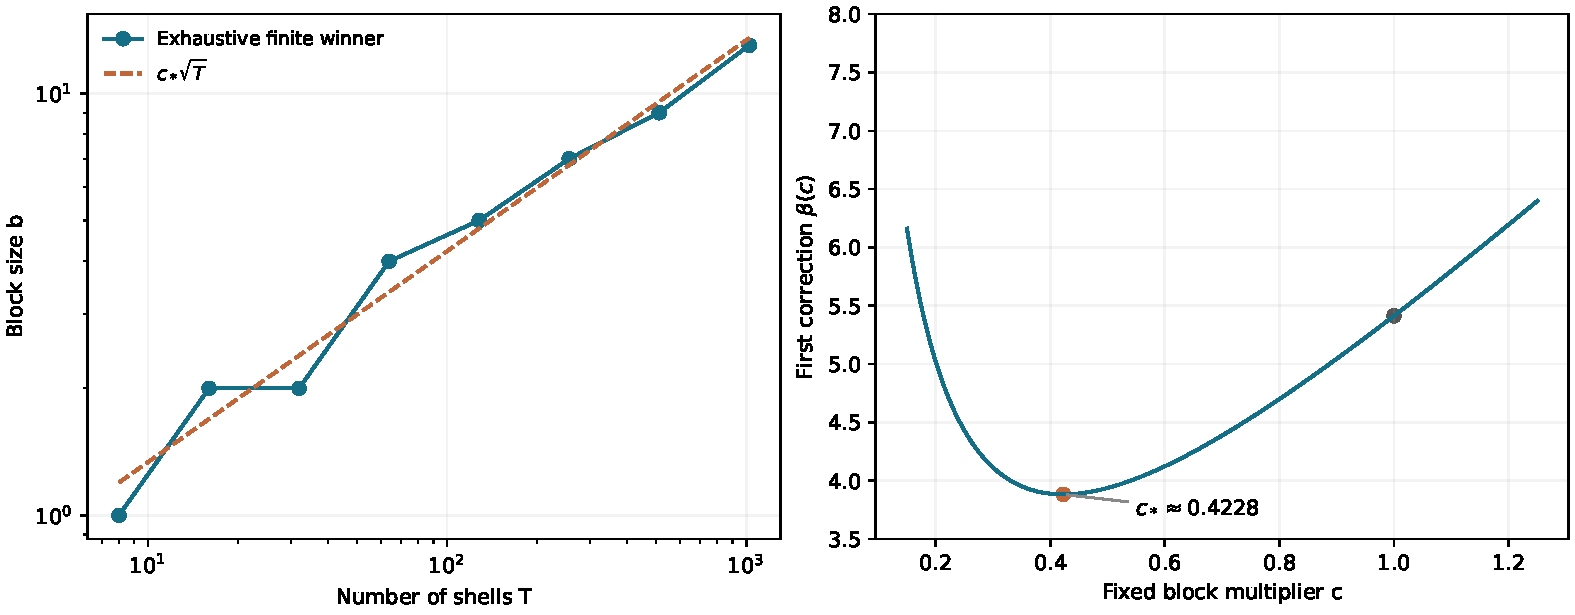
\includegraphics[width=.95\linewidth]{figures/block_discovery.pdf}
\caption{Left: exhaustive finite winners and the asymptotic guide $c_*\sqrt T$.
Right: the analytic first correction $\beta(c)$; its plotted evaluation is
numerical. This is an optimization inside a stated construction grammar,
not a graph of optimal ropelength.}
\end{figure}

\section{Reproducibility, interpretation and unresolved questions}
The repository records generator formulas, geometry and topology proofs,
independent adversarial reviews, exact endpoint data, immutable result
manifests, software versions and unsuccessful controls. The local
\texttt{publication/reproduce.py} checks bundled rational inequalities,
reproduces the main integral certificate and creates the figure. Tests and
new solver runs are explicit additional modes. No external service is needed
for the certificate once the pinned Python dependencies are installed.

The physical interpretation is $M$ separate closed filaments of radius $r$:
a unit-thickness construction scales to an admissible total contour length
$rL$. An upper construction gives sufficient length for existence, while a
lower theorem gives a necessary length. This does not describe the free-energy
minimum of one DNA molecule or a semiflexible polymer. Bending energy, tension,
thermal and hydrodynamic effects are additional models.

The outstanding research questions include a finite-$M$ comparison of
optimized blocks, variable block schedules, shell-dependent periodic pitch,
closure deformations, matching lower bounds and certified criticality.
The discovery engine currently exposes a narrower certified shell grammar;
its broader numerical extensions must not inherit the present reach theorem
without new proofs. The draft is a local publication candidate. Its original
contribution and suitability for submission require human scientific judgment;
no submission or external contact has taken place.

\paragraph{AI assistance and review.}
The research workflow used delegated Luna workers/testers and Astra adversarial
reviewers, with effective model settings logged in the repository. These are
independent implementations and adversarial computational reviews within one
AI-assisted project, not external peer review or a formal proof-assistant
verification. Authorship and publication responsibility have not been assigned.

\begin{thebibliography}{9}
\bibitem{cks} J. Cantarella, R. B. Kusner and J. M. Sullivan,
\emph{On the minimum ropelength of knots and links},
Invent. Math. 150 (2002), 257--286. \href{https://arxiv.org/abs/math/0103224}{arXiv:math/0103224}.
\bibitem{kt25} A. R. Klotz and F. Thompson, \emph{Ropelength-minimizing concentric helices and non-alternating torus knots},
Proc. R. Soc. A 481 (2025), 20250319. \href{https://doi.org/10.1098/rspa.2025.0319}{doi:10.1098/rspa.2025.0319}; equation numbering here refers to
\href{https://arxiv.org/html/2504.00861v1}{arXiv:2504.00861v1}.
\bibitem{klotz26} A. R. Klotz, \emph{Tight Bounds for Tight Links: Ropelength of $T(Q,Q)$ torus links},
J. Phys. A 59, 285201.
\href{https://doi.org/10.1088/1751-8121/ae862e}{doi:10.1088/1751-8121/ae862e};
\href{https://arxiv.org/abs/2603.02416}{arXiv:2603.02416v2}.
\bibitem{ob12} K. W. Olsen and J. Bohr, New J. Phys. 14 (2012), 023063.
\href{https://doi.org/10.1088/1367-2630/14/2/023063}{doi:10.1088/1367-2630/14/2/023063}.
\bibitem{star06} E. L. Starostin, J. Phys.: Condens. Matter 18 (2006), S187--S204.
\href{https://doi.org/10.1088/0953-8984/18/14/S04}{doi:10.1088/0953-8984/18/14/S04}.
\bibitem{atkinson19} D. W. Atkinson, C. D. Santangelo and G. M. Grason,
\emph{Constant spacing in filament bundles} (2019).
\href{https://arxiv.org/abs/1902.06325}{arXiv:1902.06325}.
\end{thebibliography}
\end{document}
